\begin{figure}[h]
\fbox{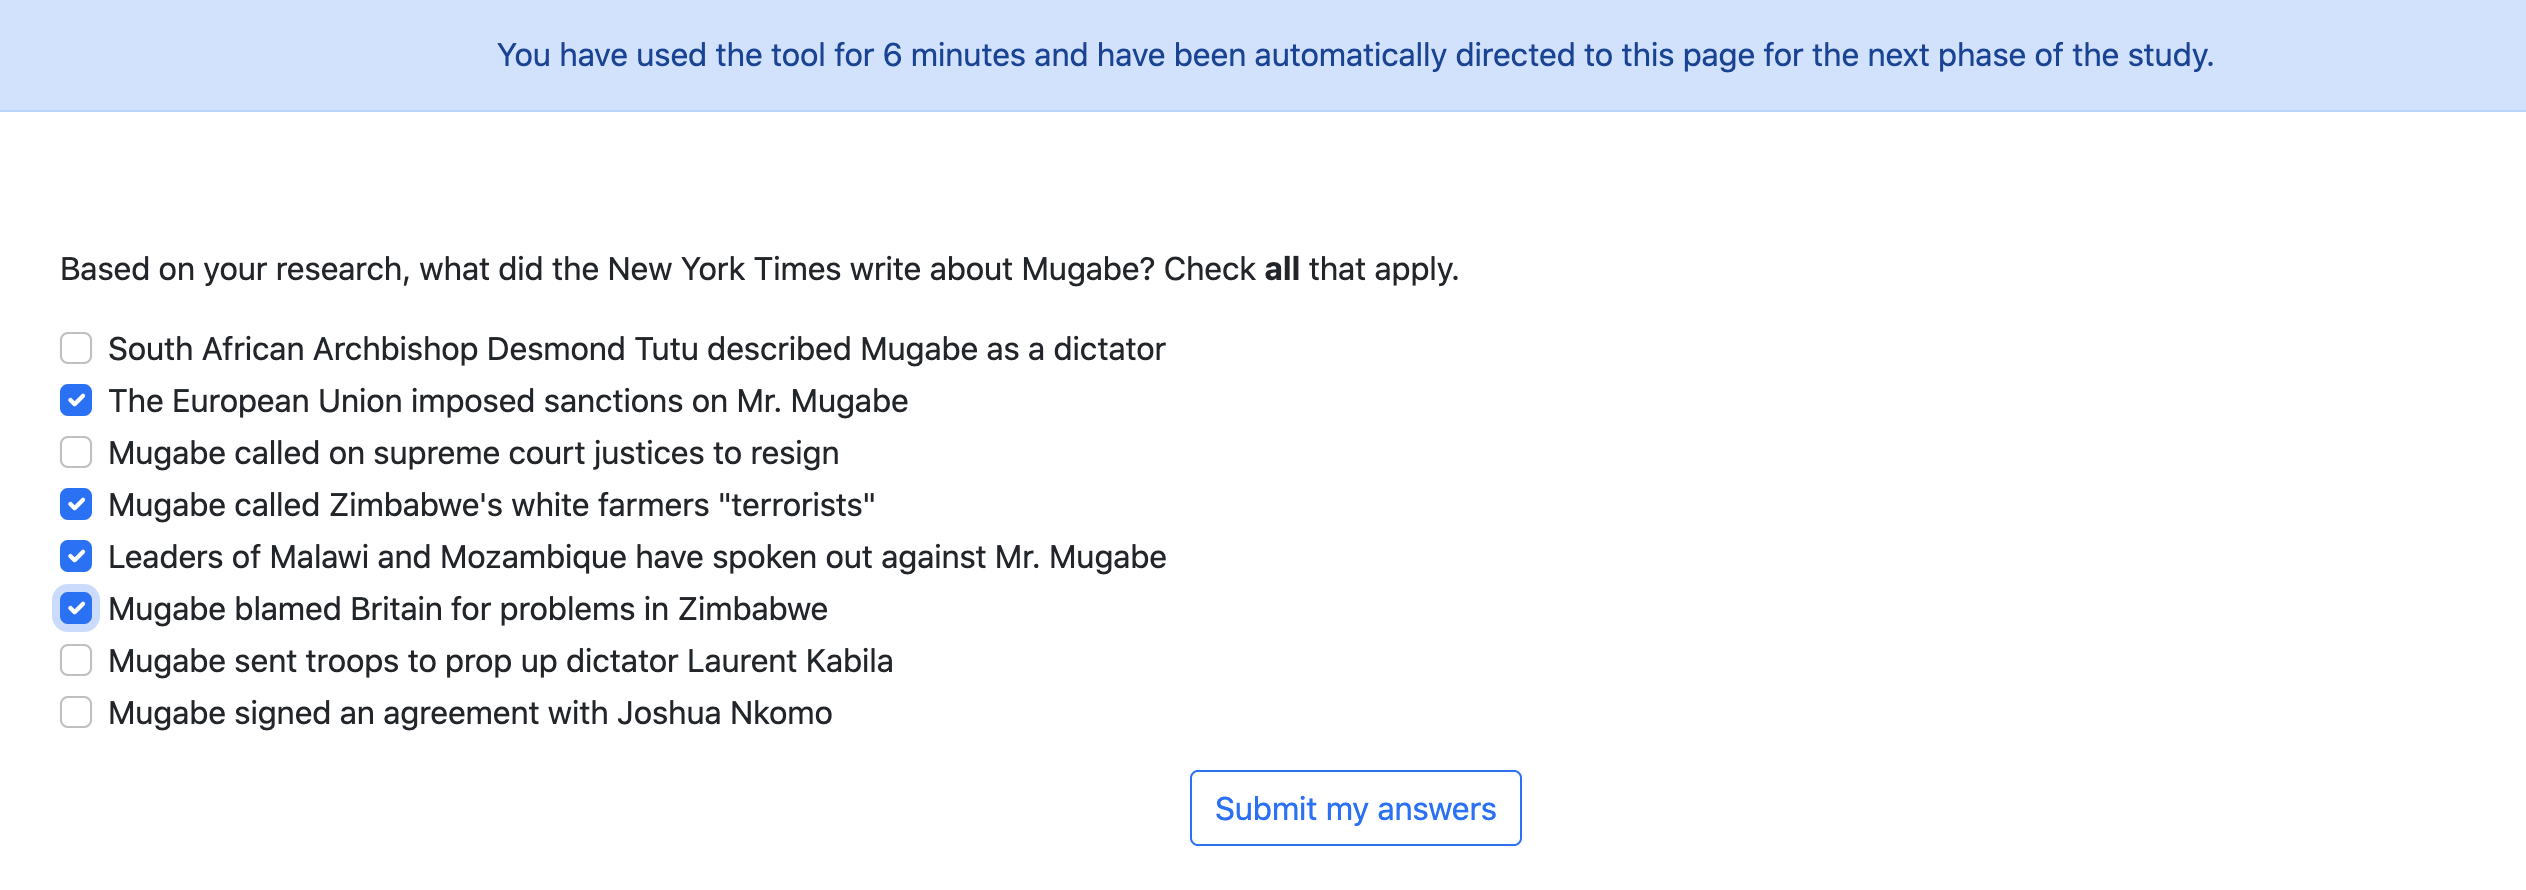
\includegraphics[width=14cm]{samples/appendix/MugabeQ.png}}
\caption{Participants answered eight true/false questions about what \textit{The New York Times} wrote about Robert Mugabe, using the form shown above. The four facts shown with checkboxes were described in editorials available to participants during the study. 
The four false facts shown without checkboxes were described in other editorials, not available to participants during the study. 
Participants who found and remembered the four facts from the corpus and who also did not incorrectly guess any of the four facts not described in the corpus scored 8 out of 8 on the reading comprehension task.
The order of questions was randomized.}
\end{figure}


\begin{figure}[h]
\fbox{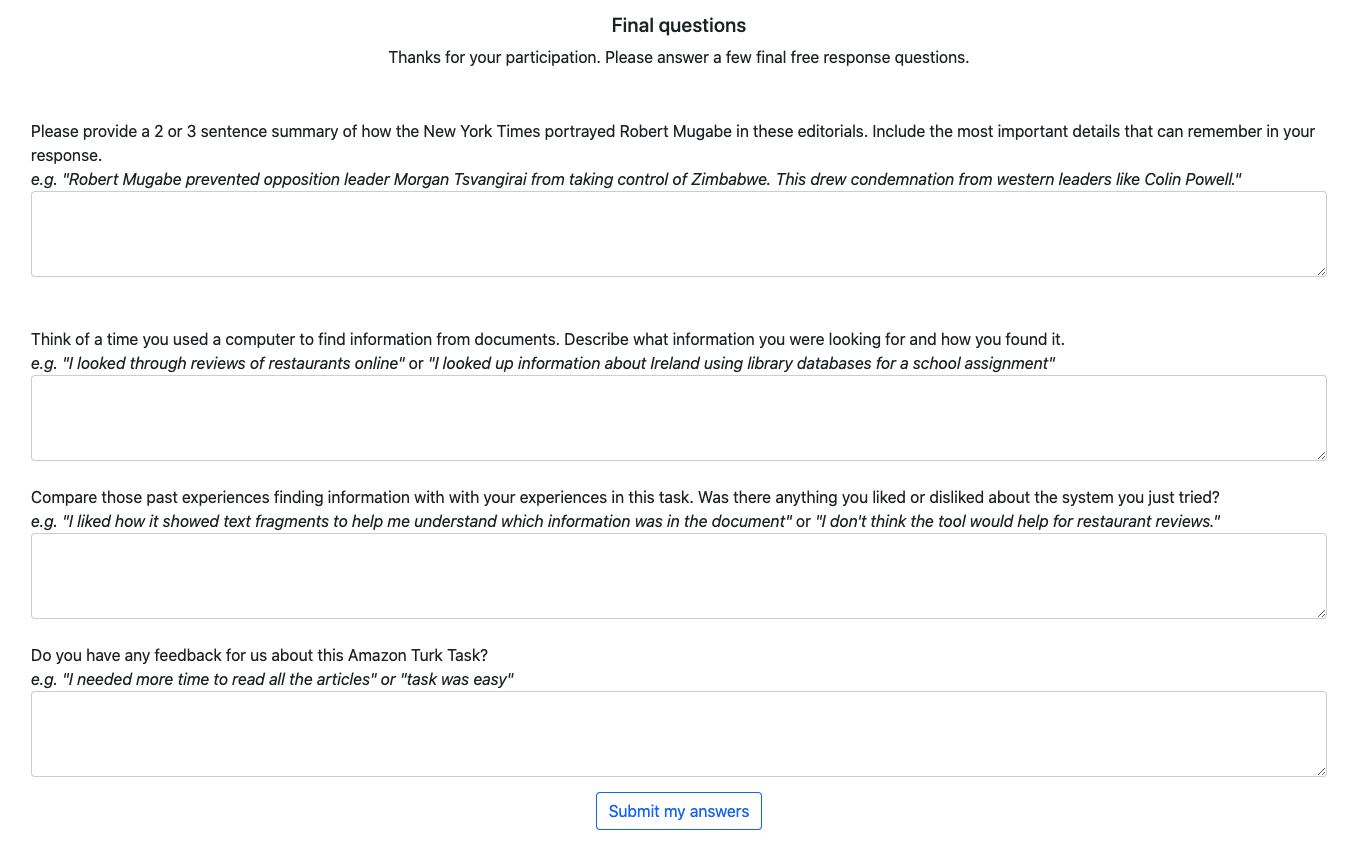
\includegraphics[width=14cm]{figures/qualQ.png}}
\caption{Qualitative questions for participants at the end of the crowd task}
\end{figure}